%%%%%%%%%%%%%%%%%%%%%%%%%%%%%%%%%%%%%%%%%%%%%%%%%%%%%%%%%%%%%%%%%%%%%
%%                                                                 %%
%% Please do not use \input{...} to include other tex files.       %%
%% Submit your LaTeX manuscript as one .tex document.              %%
%%                                                                 %%
%% All additional figures and files should be attached             %%
%% separately and not embedded in the \TeX\ document itself.       %%
%%                                                                 %%
%%%%%%%%%%%%%%%%%%%%%%%%%%%%%%%%%%%%%%%%%%%%%%%%%%%%%%%%%%%%%%%%%%%%%

%%\documentclass[referee,sn-basic]{sn-jnl}% referee option is meant for double line spacing

%%=======================================================%%
%% to print line numbers in the margin use lineno option %%
%%=======================================================%%

%%\documentclass[lineno,sn-basic]{sn-jnl}% Basic Springer Nature Reference Style/Chemistry Reference Style

%%======================================================%%
%% to compile with pdflatex/xelatex use pdflatex option %%
%%======================================================%%

%%\documentclass[pdflatex,sn-basic]{sn-jnl}% Basic Springer Nature Reference Style/Chemistry Reference Style

%%\documentclass[sn-basic]{sn-jnl}% Basic Springer Nature Reference Style/Chemistry Reference Style
\documentclass[pdflatex,sn-mathphys]{sn-jnl}% Math and Physical Sciences Reference Style
%%\documentclass[sn-aps]{sn-jnl}% American Physical Society (APS) Reference Style
%%\documentclass[sn-vancouver]{sn-jnl}% Vancouver Reference Style
%%\documentclass[sn-apa]{sn-jnl}% APA Reference Style
%%\documentclass[sn-chicago]{sn-jnl}% Chicago-based Humanities Reference Style
%%\documentclass[sn-standardnature]{sn-jnl}% Standard Nature Portfolio Reference Style
%%\documentclass[default]{sn-jnl}% Default
%%\documentclass[default,iicol]{sn-jnl}% Default with double column layout

%%%% Standard Packages
%%<additional latex packages if required can be included here>
%%%%

%%%%%=============================================================================%%%%
%%%%  Remarks: This template is provided to aid authors with the preparation
%%%%  of original research articles intended for submission to journals published 
%%%%  by Springer Nature. The guidance has been prepared in partnership with 
%%%%  production teams to conform to Springer Nature technical requirements. 
%%%%  Editorial and presentation requirements differ among journal portfolios and 
%%%%  research disciplines. You may find sections in this template are irrelevant 
%%%%  to your work and are empowered to omit any such section if allowed by the 
%%%%  journal you intend to submit to. The submission guidelines and policies 
%%%%  of the journal take precedence. A detailed User Manual is available in the 
%%%%  template package for technical guidance.
%%%%%=============================================================================%%%%

\jyear{2022}%

%% as per the requirement new theorem styles can be included as shown below
\theoremstyle{thmstyleone}%
\newtheorem{theorem}{Theorem}%  meant for continuous numbers
%%\newtheorem{theorem}{Theorem}[section]% meant for sectionwise numbers
%% optional argument [theorem] produces theorem numbering sequence instead of independent numbers for Proposition
\newtheorem{proposition}[theorem]{Proposition}% 
%%\newtheorem{proposition}{Proposition}% to get separate numbers for theorem and proposition etc.

\theoremstyle{thmstyletwo}%
\newtheorem{example}{Example}%
\newtheorem{remark}{Remark}%

\theoremstyle{thmstylethree}%
\newtheorem{definition}{Definition}%

\raggedbottom
%%\unnumbered% uncomment this for unnumbered level heads

\begin{document}

\title[Cervical Spine Fracture Detection and Localization]{Cervical Spine Fracture Detection and Localization}

%%=============================================================%%
%% Prefix	-> \pfx{Dr}
%% GivenName	-> \fnm{Joergen W.}
%% Particle	-> \spfx{van der} -> surname prefix
%% FamilyName	-> \sur{Ploeg}
%% Suffix	-> \sfx{IV}
%% NatureName	-> \tanm{Poet Laureate} -> Title after name
%% Degrees	-> \dgr{MSc, PhD}
%% \author*[1,2]{\pfx{Dr} \fnm{Joergen W.} \spfx{van der} \sur{Ploeg} \sfx{IV} \tanm{Poet Laureate} 
%%                 \dgr{MSc, PhD}}\email{iauthor@gmail.com}
%%=============================================================%%

\author{\fnm{Naman} \sur{Raghuvanshi}}\email{nvr5386@psu.edu}

\author{\fnm{Siddharth} \sur{Rayabharam}}\email{nqr5356@psu.edu}

\author{\fnm{Sumant} \sur{Suryawanshi}}\email{szs7220.psu.edu}


%%==================================%%
%% sample for unstructured abstract %%
%%==================================%%

\abstract{\textbf{Purpose:} To develop a deep learning model for the detection and localization of cervical spine fractures in the axial CT scans. 

\textbf{Methods:} We use the dataset consisting of cervical spine CT scans provided by the Radiological Society of North America (RSNA). The dataset consists of 3000 studies of individual patients for the training and testing combined. Out of these 3000 patient studies, 83 of these studies also contains segmentation data. Additionally, for x studies the dataset contains bounding box coordinates data. The dataset population is split into 90\% for training and 10\% for validation. We use EfficientNetV2\cite{DBLP:conf/icml/TanL21} to learn the segmentation, YOLOv5 model for detecting the fractures and drawing bounding boxes around the fracture area.

\textbf{Results:} The segmentation model predicts the vertebrae label with the accuracy of 95.13\% whereas the fracture detection model predicts fractures with an accuracy of 94\%. The fracture detection model also draws bounding boxes localizing the fractures and provides the objectiveness of the prediction.

\textbf{Conclusion:} We have demonstrated that deep learning models are able to provide good fracture detection predictions and localization from the CT radiographs. We have shown that the CNNs holds promise at both worklist prioritization and assisting radiologists in cervical spine fracture detection on CT radiographs.
}
% Fracture detection is a crucial part of a computer-aided medical system. In this project, we provide a unified technique for the detection and localization of cervical spine fractures from the axial CT scans of the cervical spine. This project is meant to speed up the diagnosis and is not a substitution of the medical experts. In this project, a model first segments the examination slices from C1 to C7 and detects the presence of the fracture in the slice. Moreover, another model has been proposed to localize the line-of-break using bounding boxes for easy visualization of the fracture.

%%================================%%
%% Sample for structured abstract %%
%%================================%%

% \abstract{\textbf{Purpose:} The abstract serves both as a general introduction to the topic and as a brief, non-technical summary of the main results and their implications. The abstract must not include subheadings (unless expressly permitted in the journal's Instructions to Authors), equations or citations. As a guide the abstract should not exceed 200 words. Most journals do not set a hard limit however authors are advised to check the author instructions for the journal they are submitting to.
% 
% \textbf{Methods:} The abstract serves both as a general introduction to the topic and as a brief, non-technical summary of the main results and their implications. The abstract must not include subheadings (unless expressly permitted in the journal's Instructions to Authors), equations or citations. As a guide the abstract should not exceed 200 words. Most journals do not set a hard limit however authors are advised to check the author instructions for the journal they are submitting to.
% 
% \textbf{Results:} The abstract serves both as a general introduction to the topic and as a brief, non-technical summary of the main results and their implications. The abstract must not include subheadings (unless expressly permitted in the journal's Instructions to Authors), equations or citations. As a guide the abstract should not exceed 200 words. Most journals do not set a hard limit however authors are advised to check the author instructions for the journal they are submitting to.
% 
% \textbf{Conclusion:} The abstract serves both as a general introduction to the topic and as a brief, non-technical summary of the main results and their implications. The abstract must not include subheadings (unless expressly permitted in the journal's Instructions to Authors), equations or citations. As a guide the abstract should not exceed 200 words. Most journals do not set a hard limit however authors are advised to check the author instructions for the journal they are submitting to.}

\keywords{Cervical Spine, Fracture Detection, Deep Learning}

%%\pacs[JEL Classification]{D8, H51}

%%\pacs[MSC Classification]{35A01, 65L10, 65L12, 65L20, 65L70}

\maketitle
\section{Introduction}\label{sec1}

Cervical spine injury is very common injury with more than 3 million cases per year that are being evaluated for cervical spine injury in North America\cite{Milby:2008tt}. In United States, more than 1 million patients with blunt force injury are suspected to suffer cervical spine injury\cite{Minja:2018ud}. Since cervical spine injury is associated with high morbidity and mortality, quick diagnosis of the injury is crucial. Any delay in diagnosis may result in devastating consequences for the patient. So, any additional aid to the radiologists can reduce the morbidity or mortality of the patient.

In recent years, a machine deep learning technique known as deep convolutional neural network (DCNN) has been applied to image recognition tasks. DCNN's are well suited for images. So, they have been used extensively in the field of medicine to classify medical images. 

In past few years, there have been many studies that have tried to use DCNN\cite{Olczak:2017aa}\cite{Kim:2018aa}\cite{Chung:2018aa} on medical radiographs. In these studies, the reference standard for the training and testing images was based on the assessment of human readers determining which were visible, only within a radiograph. Many radiologist fail to detect "occult fracture" because of the difficulty in detecting such fracture in a radiograph. These extraction methodologies could adversely influence the classification accuracy and occult fracture being assessed as a “non-fracture case”. A proficient algorithm may help identify and triage studies for the radiologist to review more urgently, helping to ensure faster diagnoses.

The purpose of our study is to develop an automated deep learning system for detecting cervical spine fractures using CT a gold standard annotated by radiologists, and to evaluate the diagnostic performance inclusive of the experienced readers in detecting cervical spine fractures on radiographs. 

\section{Literature Review}\label{litrev}

Many studies have been conducted to utilize deep learning techniques in tele-medicine field. We have adequate amount of literature that is relevant to our project. However, The CNN model proposed by J.E. Small et al. to detect the cervical spine fracture detection with the accuracy of 92\%\cite{Small:2021aa}. According to their study, the radiologists are 95\% accurate in the cervical spine fracture detection. The fractures missed by the proposed model and the radiologists were similar by level and location which is mostly included fractures which are obscured by CT beam attenuations. Yee Liang Thian et al.\cite{Thian:2019aa} have implemented Inception-ResNet Faster R-CNN  architecture to detect and localize the fractures on wrist radiographs. The model detected and correctly localized 310 (91.2\%) of 340 and 236 (96.3\%) of 245 of all radius and ulna fractures on the frontal and lateral views, respectively.

Yoga Dwi Pranata et al. have implemented ResNet and VGG for automated classification and detection of calcaneus fracture in CT images\cite{PRANATA201927}. The bone fracture detection algorithm incorporated fracture area matching using the speeded-up robust features (SURF) method, Canny edge detection, and contour tracing. Their results showed that ResNet was comparable in accuracy, of 98\%, to the VFF network for bone fracture classification but achieved better performance. Tsubasa Mawatari et al. have studied about the effect of deep convolutional networks on radiologists performance in the detection of hip fractures on digital pelvic radiograph. According to the study, the average AUC of the 7 readers was 0.832. The AUC of DCNN alone was 0.905. The average AUC of the 7 readers with DCNN outputs was 0.876. The AUC of readers with DCNN output were higher than those without\cite{Mawatari:2020aa}.

\section{Methodology}\label{sec2}

\subsection{Dataset and Study Population}\label{subsec2}

We use the dataset consisting of cervical spine CT scans provided by the Radiological Society of North America (RSNA)\cite{rsna-url}. The dataset we are using is made up of roughly 3000 CT studies, from twelve locations and across six continents. Spine radiology specialists have provided annotations to indicate the presence, vertebral level and location of any cervical spine fractures. Each radiology study consists of multiple dcm files. A dcm file follows the Digital Imaging and Communications in Medicine (DICOM) format. It is the standard format used for storing medical images and related metadata. It dates back to 1983, although it has been revised many times. Out of these 3000 patient studies, 83 of these studies also contains segmentation data. Additionally, for x studies the dataset contains bounding box coordinates data. The dataset population is split into 90\% for training and 10\% for validation. The distribution of fractured and non-fractured dataset in the dataset is shown in the below two graphs.

\begin{figure}[H]
\centering
 \begin{minipage}[c]{1\textwidth}
    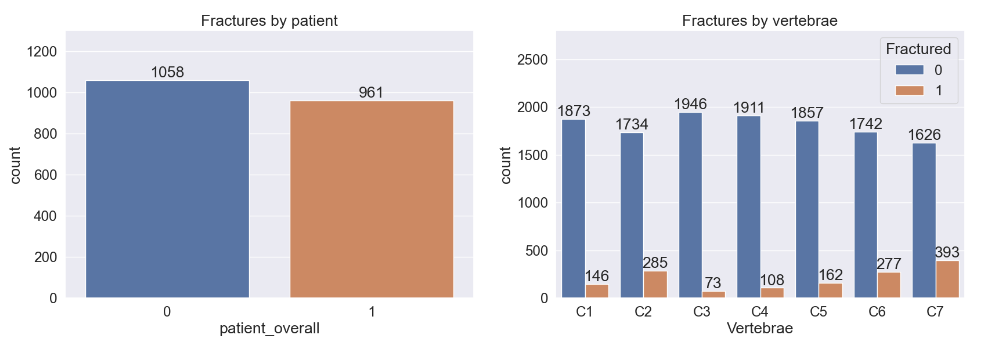
\includegraphics[width=\textwidth]{fracture-distribution}
    \caption{\centering\footnotesize{a) Number of patients with fractures (blue) and without fractures (red). b) Fracture distribution among the vertebrae C1, C2, C3, C4, C5, C6 and C7. }}
    \label{fig:mesh1}
\end{minipage}
\end{figure}

\subsection{Data Pre-processing}

\subsubsection{Windowing}

Every CT radiograph contains details of multiple tissues. To highlight only certain anatomical features of the radiograph we use \emph{windowing}. Windowing, also known as grey-level mapping, contrast stretching, histogram modification or contrast enhancement is the process in which the CT image greyscale component of an image is manipulated via the CT numbers. The CT numbers are represented in terms of Hounsfield Units (HU).

\vspace*{-5mm}
\begin{figure}[H]
 \begin{minipage}[c]{1\textwidth}
 \centering
    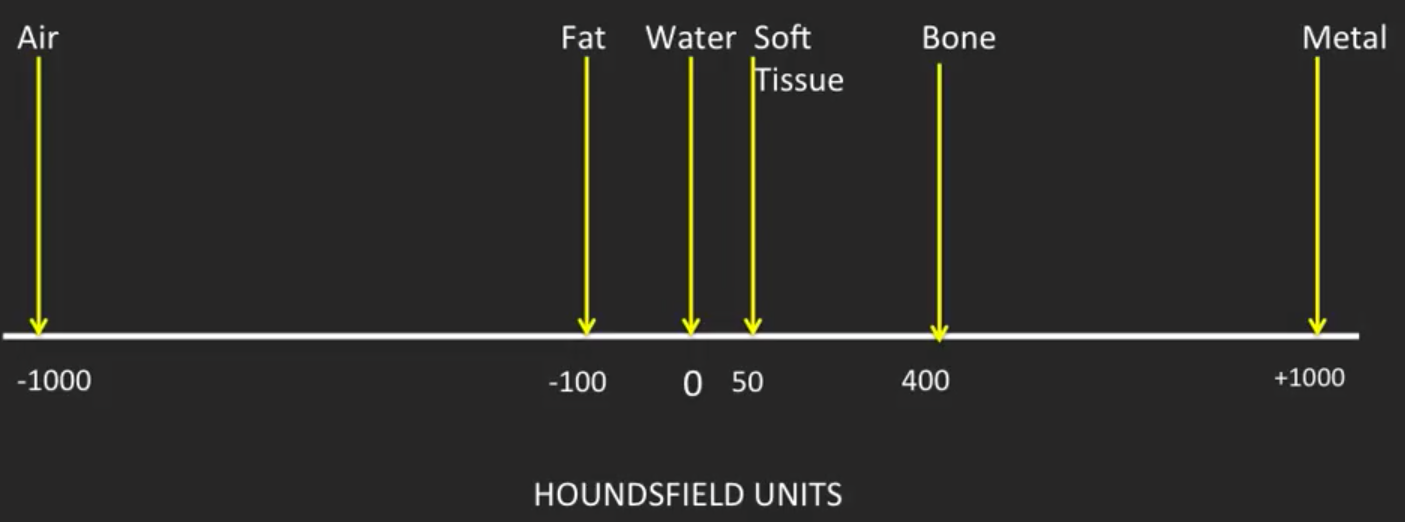
\includegraphics[width=0.8\textwidth]{hu}
    \caption{\centering\footnotesize{ Hounsfield Units for different mediums. }}
    \label{fig:mesh2}
\end{minipage}
\end{figure}

\vspace*{-5mm}
The CT scans are manipulated using \emph{window width} and \emph{window level}. The window width is the measure of range of different CT numbers. The Window Level (WL) refers to the window centre or midpoint HU value that is represented on the window setting. For our project we use window width of 1800 and window level of 400\cite{DBLP:journals/corr/abs-1812-00572}.

\vspace*{-5mm}
\begin{figure}[H]
\centering
\begin{minipage}[c]{0.5\textwidth}
    \centering
    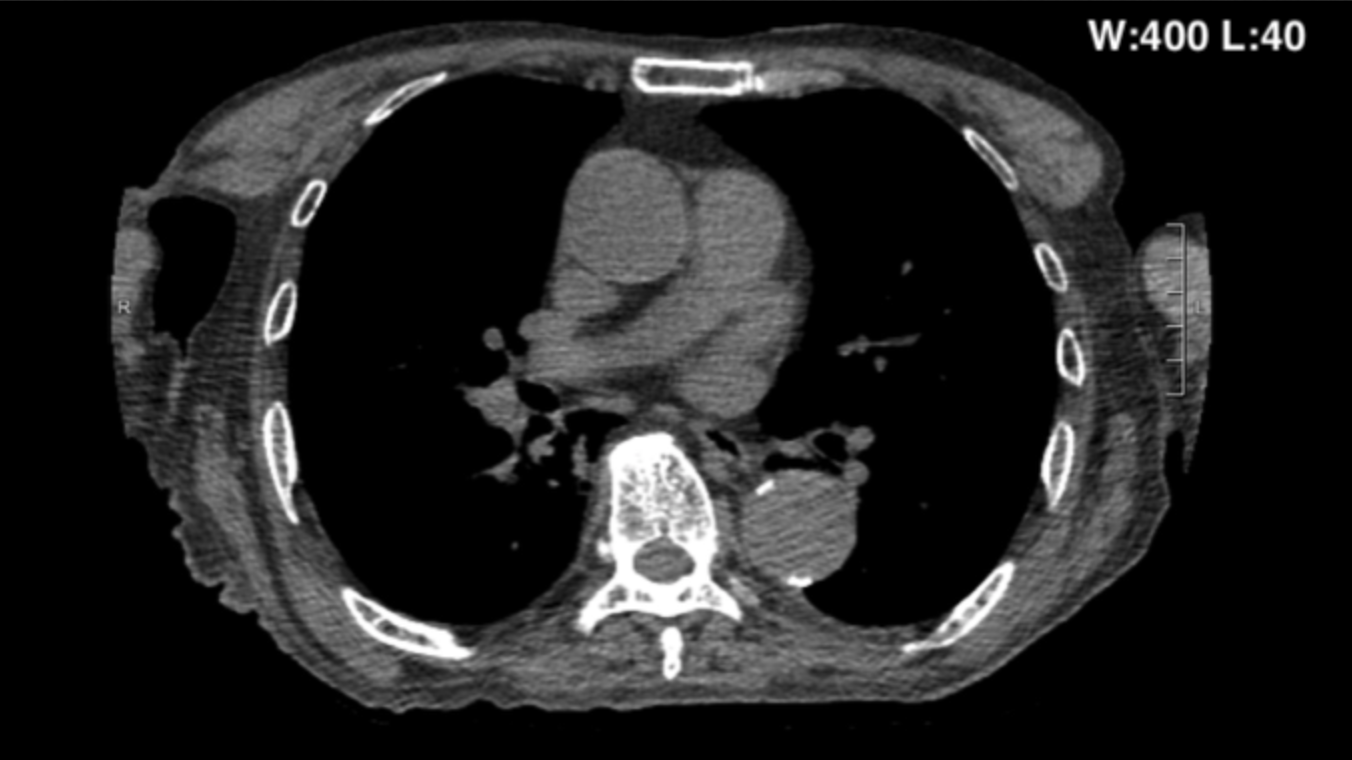
\includegraphics[height=0.55\textwidth]{windowing-impact-1}
    
    \label{fig:mesh3.1}
\end{minipage}\hfill
\begin{minipage}[c]{0.5\textwidth}
    \centering
    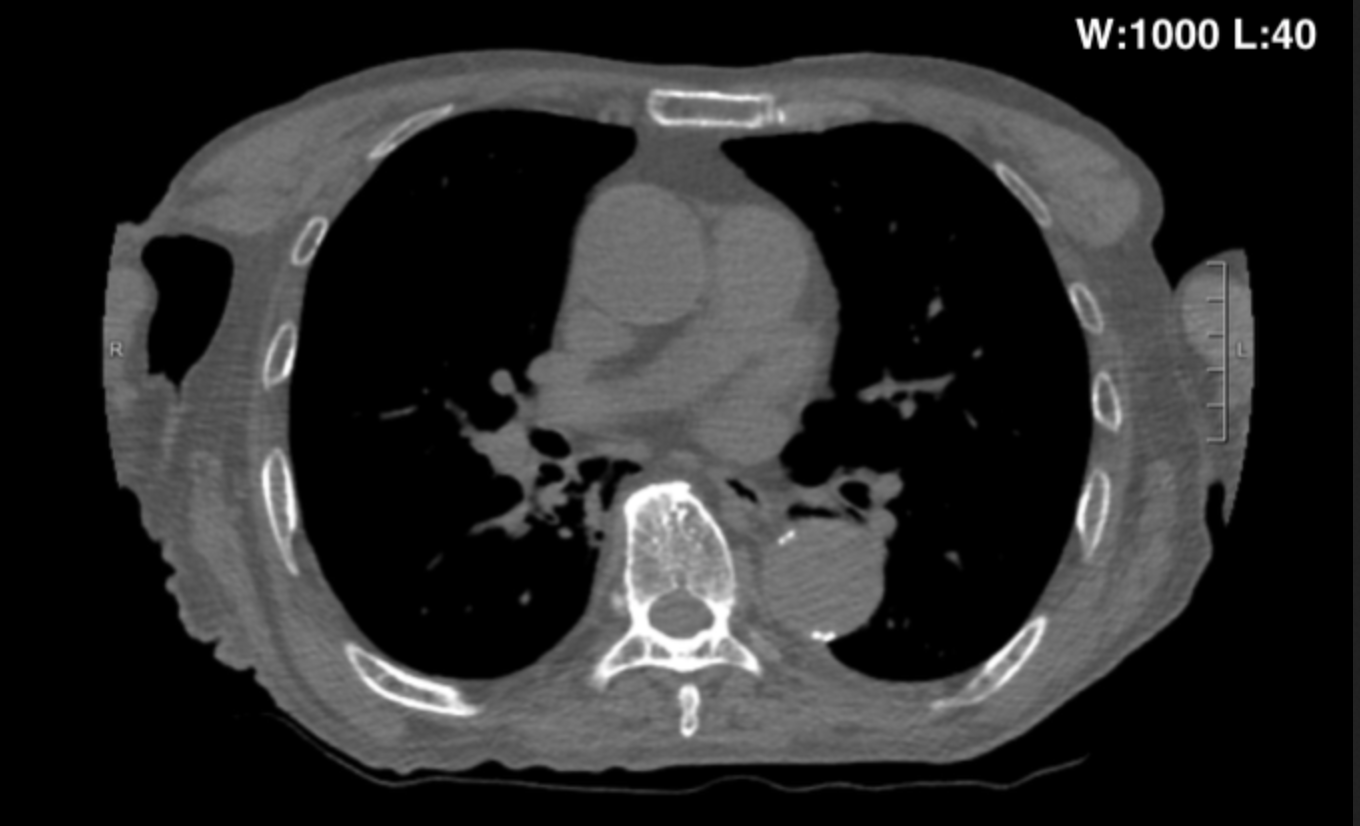
\includegraphics[height=0.55\textwidth]{windowing-impact-2}
    \label{fig:mesh3.2}
\end{minipage}
\caption{\centering\footnotesize{Impact of window width on the appearnace of a CT scan. }}
\end{figure}
\vspace*{-10mm}

\subsubsection{Resizing}

Almost all images have size 512x512. We therefore resized the other dimension images to  size 512x512.

\vspace*{-5mm}
\begin{figure}[H]
 \begin{minipage}[c]{1\textwidth}
 \centering
    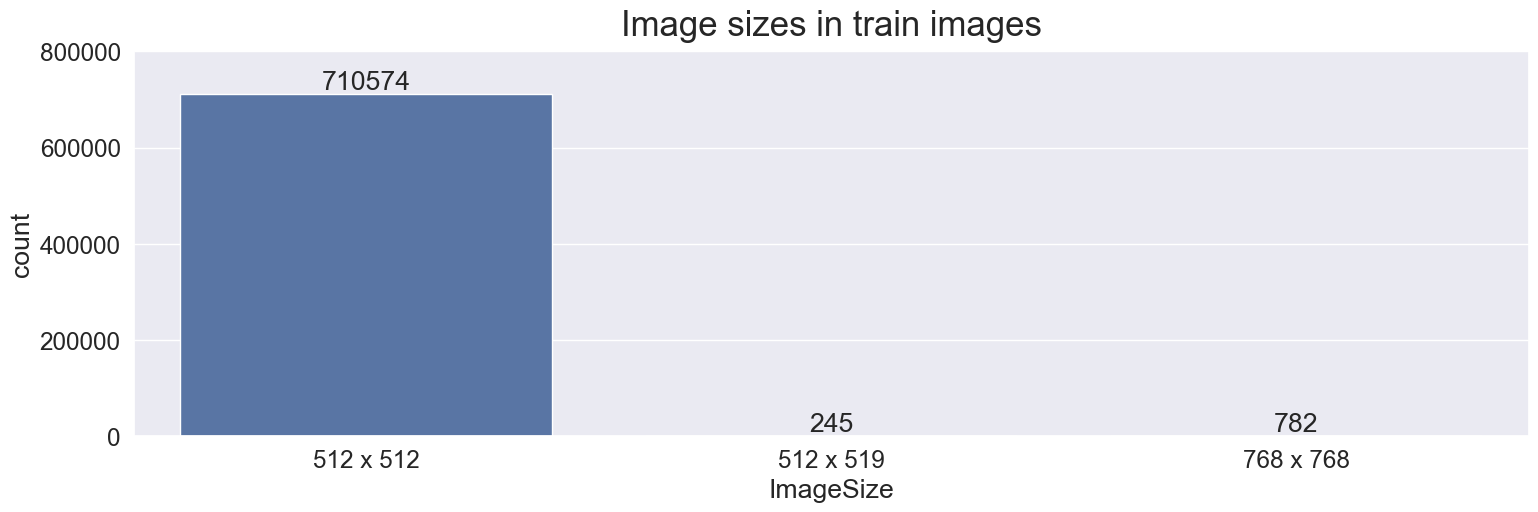
\includegraphics[width=0.8\textwidth]{resizing}
    \caption{\centering\footnotesize{ Image size in train images. }}
    \label{fig:mesh4}
\end{minipage}
\end{figure}

\subsection{Detection}\label{subsec1}

We perform fracture detection in the two phases. The first phase is segmentation of all the available study slices of CT radiographs whereas the second phase is fracture detection and localization, which is done by displaying bounding boxes covering fractures. The flow of the training dataset is described in the below figure.

\begin{figure}[H]
 \begin{minipage}[c]{1\textwidth}
 \centering
    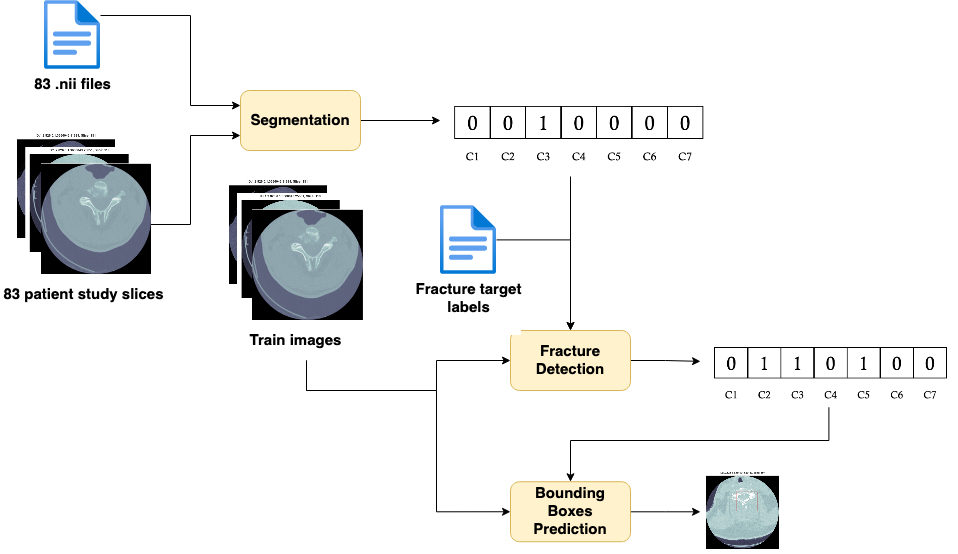
\includegraphics[width=\textwidth]{methodology}
    \caption{\centering\footnotesize{ Data flow in model training. }}
    \label{fig:flow}
\end{minipage}
\end{figure}

\subsubsection{Segmentation}

Segmentation involves classification of CT radiographs into C1 to C7 labels. Using the 83 studies which have segmentation data, we train Random Forest classifier\cite{SEG:RandForest} and EfficientNetV2\cite{DBLP:conf/icml/TanL21}. First we extract vertebrae targets from 83 segmentation files and use them for training. The trained segmentation models take the slices as the input and output the one-hot encoded labels for each slice indicating the vertebrae the slice belongs. Correct vertebrae labels are essential when training the fracture prediction model. 

\subsubsection{Fracture Detection and Localization}

The fracture detection data consists of data indicating which vertebrae has fracture in a particular CT examination (each CT examination contains many slices). Therefore, we store the labels predicted by the segmentation model and merge them with the fracture detection data to obtain the information if a slice in an examination has fracture or not. The model is then trained on this merged data to predict fractures in a particular slice of a CT examination. EfficientNetV2 and YOLOv5\cite{glenn_jocher_2022_7347926}. 

Localization here, refers to highlighting or bounding the fracture with box in the CT radiograph. EfficientNetV2 only produces the fracture detections and not the localization whereas the YOLOv5 model predicts the fractures and localizes the fractures. YOLOv5 model also provides the confidence measure of fracture in the bounding box.

\section{Results}\label{sec3}

\subsection{Segmentation}

From Table 1, we can see that EfficientNet performs well compared to the Random Forest Classifier. EfficientNetV2 is a new family of convolutional networks that have faster training speed and better parameter efficiency than previous models. To develop these models, a combination of training-aware neural architecture search and scaling was used to jointly optimize training speed and parameter efficiency. The models were searched from the search space enriched with new ops such as Fused-MBConv\cite{Fused-MBConv}. Experiments show that EfficientNetV2 models train much faster than state-of-the-art models while being up to 6.8x smaller. With transfer learning, EfficientNetV2 significantly outperforms previous models on ImageNet and CIFAR/Cars/Flowers datasets\cite{DBLP:conf/icml/TanL21}. By pretraining on the same ImageNet21k, EfficientNetV2 achieves 87.3\% top-1 accuracy on ImageNet ILSVRC2012, outperforming the recent ViT by 2.0\% accuracy while training 5x-11x faster using the same computing resources.

\begin{table}[!h]
\centering
\begin{tabular}{c|c|c}
\textbf{Vetebrae} & \textbf{\begin{tabular}[c]{@{}c@{}}Random Forest \\ Classifier\end{tabular}} & \textbf{EfficientNetV2} \\ \hline
C1 & 0.8891 & 0.9621 \\ \hline
C2 & 0.8898 & 0.9409 \\ \hline
C3 & 0.8962 & 0.9559 \\ \hline
C4 & 0.8952 & 0.9605 \\ \hline
C5 & 0.8893 & 0.9482 \\ \hline
C6 & 0.8713 & 0.9450 \\ \hline
C7 & 0.8576 & 0.9465 \\ \hline
Overall & 0.8841 & 0.9513 \\ \hline
\end{tabular}
\caption[]
	{\centering\small Accuracies of the models for the segmentation}
\end{table}

The EffNetV2 model is validated using the k-fold ($k=5$) validation technique. The validation loss and accuracy of the model for $k$ different runs.

\begin{figure}[H]
 \begin{minipage}[c]{0.5\textwidth}
 \centering
    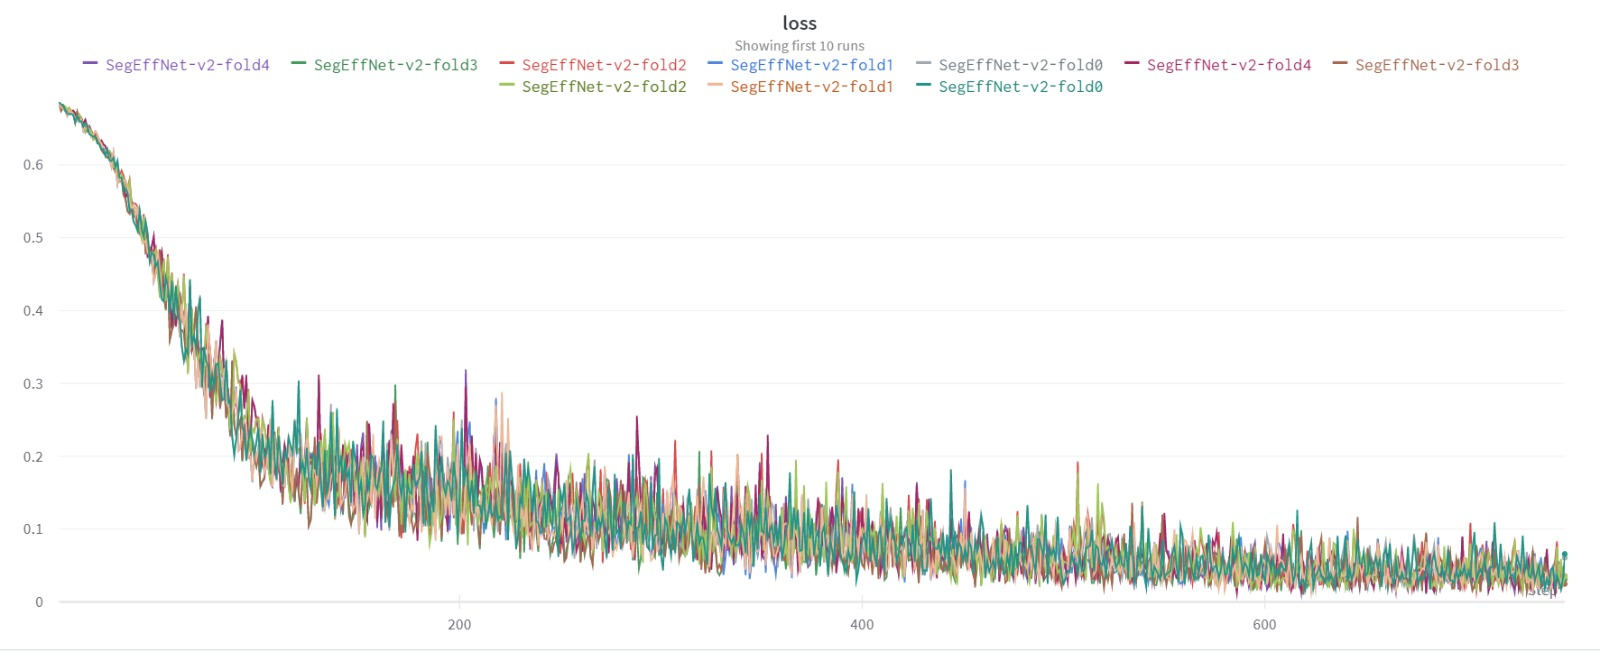
\includegraphics[width=\textwidth]{seg_loss}
    \label{fig:mesh5.1}
\end{minipage}
\begin{minipage}[c]{0.5\textwidth}
 \centering
    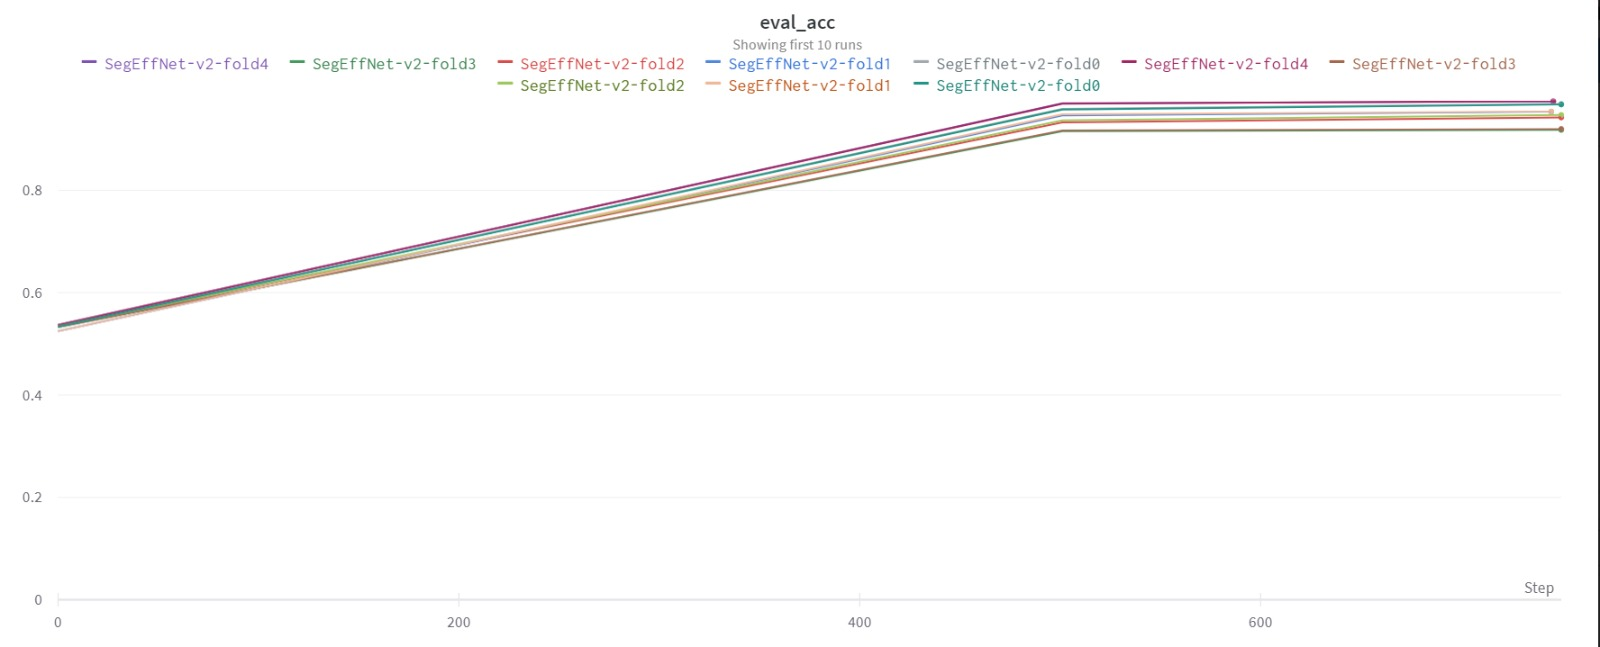
\includegraphics[width=\textwidth]{seg_eval_acc}
    \label{fig:mesh5.2}
\end{minipage}
\caption{\centering\footnotesize{ The validation loss and accuracy of EffNetV2 for differnt runs. }}
\end{figure}

Below are the prediction probabilities of 3 study samples for each vertebrae.

\begin{figure}[H]
\begin{minipage}[c]{1\textwidth}
 \centering
    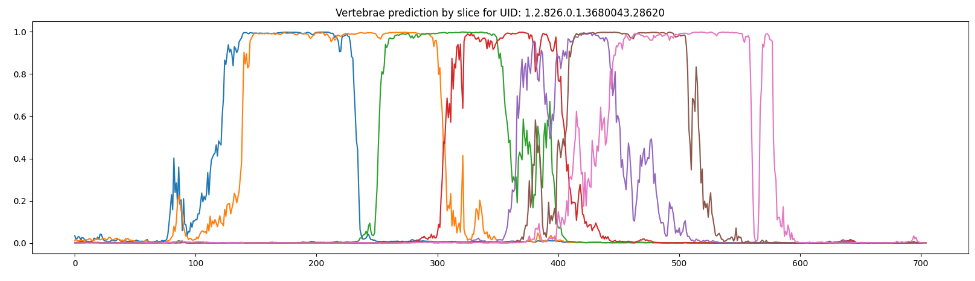
\includegraphics[width=\textwidth]{vertebrae-prediction-1}
    \label{fig:mesh5.1}
\end{minipage}
\begin{minipage}[c]{1\textwidth}
 \centering
    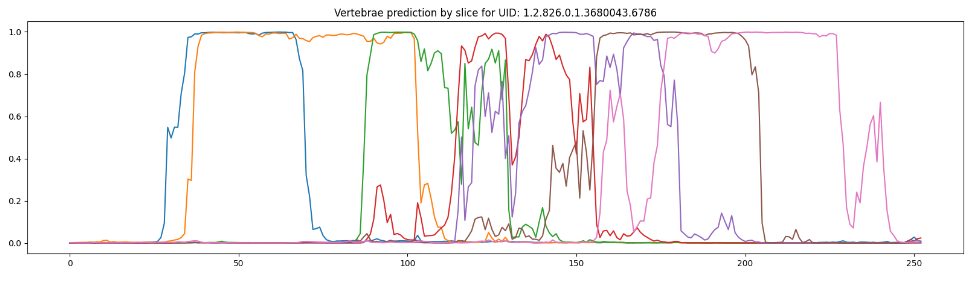
\includegraphics[width=\textwidth]{vertebrae-prediction-2}
    \label{fig:mesh5.2}
\end{minipage}
\begin{minipage}[c]{1\textwidth}
 \centering
    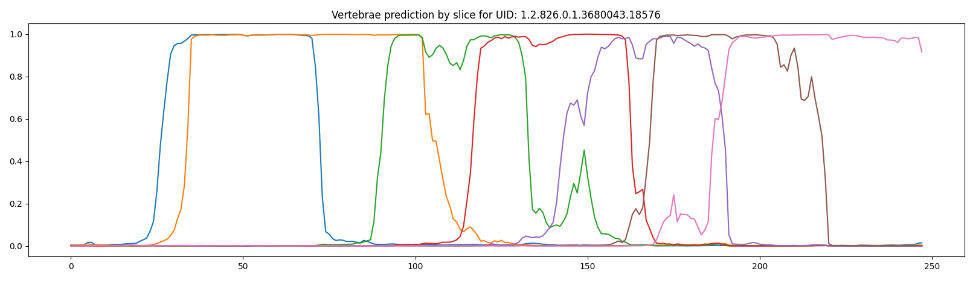
\includegraphics[width=\textwidth]{vertebrae-prediction-3}
    \label{fig:mesh5.3}
\end{minipage}
\caption{\centering\footnotesize{ Vertebrae prediction by slice for 3 study samples. }}
\end{figure}

\subsection{Fracture Detection}\label{subsubsec2}

EffNetV2 and YOLOv5 have been trained on the dataset to detect fractures on the CT radiographs. The results of these two models are discussed below

\subsubsection{EffNetV2}

Need to EffNet results here


\subsubsection{YOLOv5}

The accuracy acheived by the YOLOv5 model is 94\% in fracture detection and localization. Table 2 shows the performance metrics of the model. Similarly, Table 3 shows the average performance of the model.

\begin{table}[!h]
\centering
\begin{tabular}{|ccccc|}\hline
 & \textbf{Precision} & \textbf{Recall} & \textbf{f1-score} & \textbf{support} \\\hline
\textbf{Normal} & 0.73 & 0.84 & 0.78 & 200 \\ \hline
\textbf{Fractured} & 0.98 & 0.96 & 0.97 & 1444\\\hline
\end{tabular}
\caption{\centering\footnotesize{ Performance metrics }}
\end{table}

\begin{table}[!h]
\centering
\begin{tabular}{|ccccc|}\hline
 & \textbf{Precision} & \textbf{Recall} & \textbf{f1-score} & \textbf{support} \\\hline
\textbf{Accuracy} &  &  &  & 1644 \\\hline
\textbf{Macro Avg} & 0.85 & 0.90 & 0.88 & 1644 \\\hline
\textbf{Weighted Avg} & 0.95 & 0.94 & 0.95 & 1644\\\hline
\end{tabular}
\caption{\centering\footnotesize{ Average performance metrics }}
\end{table}




\section{Future Works}\label{sec12}

Future works can implement include fracture highlighting which will create a highlight on top of the predicted bone crack. We intend to use the study to detect cracks in concrete structures using deep learning and image manipulation techniques\cite{su14138117}. 

On the other hand, current flow of prediction can be improved by creating an ensemble of two models or by create a single model to perform segmentation, fracture detection and localization tasks. Further improvements can be made in segmentation model to impose monotonicity on the predictions i.e., to reduce predictions where the slice is predicted to be in two or more vertebrae.

\section{Conclusion}\label{sec13}

We have demonstrated that deep learning models are able to provide good fracture detection predictions and localization from the CT radiographs. The results have shown the feasibility of the above mentioned models to perform cervical spine fracture detection with 95\% in segmentation and 94\% in fracture detection and localization. This that the CNNs holds promise at both worklist prioritization and assisting radiologists in cervical spine fracture detection on CT radiographs.

\newpage


%%===========================================================================================%%
%% If you are submitting to one of the Nature Portfolio journals, using the eJP submission   %%
%% system, please include the references within the manuscript file itself. You may do this  %%
%% by copying the reference list from your .bbl file, paste it into the main manuscript .tex %%
%% file, and delete the associated \verb+\bibliography+ commands.                            %%
%%===========================================================================================%%

\bibliography{sn-bibliography}% common bib file
%% if required, the content of .bbl file can be included here once bbl is generated
%\input sn-report.bib

%% Default %%
%%\input sn-sample-bib.tex%

\end{document}
